\chapter{Appendix}
\section{Tallier Implementation}
\section{ESP32 Guardian Implementation}
\section{ESP32 Guardian Documentation}

\section{Error Message}
\begin{lstlisting}[language=Python, label={lst:proof}, breaklines=true, breakatwhitespace=false, linewidth=\textwidth, caption={Tallier receives Decryption with invalid Chaum-Pedersen proof}]
[5546:2025-02-24 10:38:36,167]:WARNING:decryption_share.py.is_valid:#L129: CiphertextDecryptionSelection is_valid failed for guardian: 083af2b6253c selection: yes-selection with invalid proof
[5546:2025-02-24 10:38:36,178]:WARNING:decrypt_with_shares.py.decrypt_selection_with_decryption_shares:#L182: share: yes-selection has invalid proof or recovered parts
[5546:2025-02-24 10:38:36,188]:WARNING:decrypt_with_shares.py.decrypt_contest_with_decryption_shares:#L146: could not decrypt contest referendum-single-vote with selection yes-selection
[5546:2025-02-24 10:38:36,200]:WARNING:decrypt_with_shares.py.decrypt_tally:#L66: contest: referendum-single-vote failed to decrypt with shares
\end{lstlisting}
\section{Additional Figures} 
\begin{figure}[h!]
    \centering
    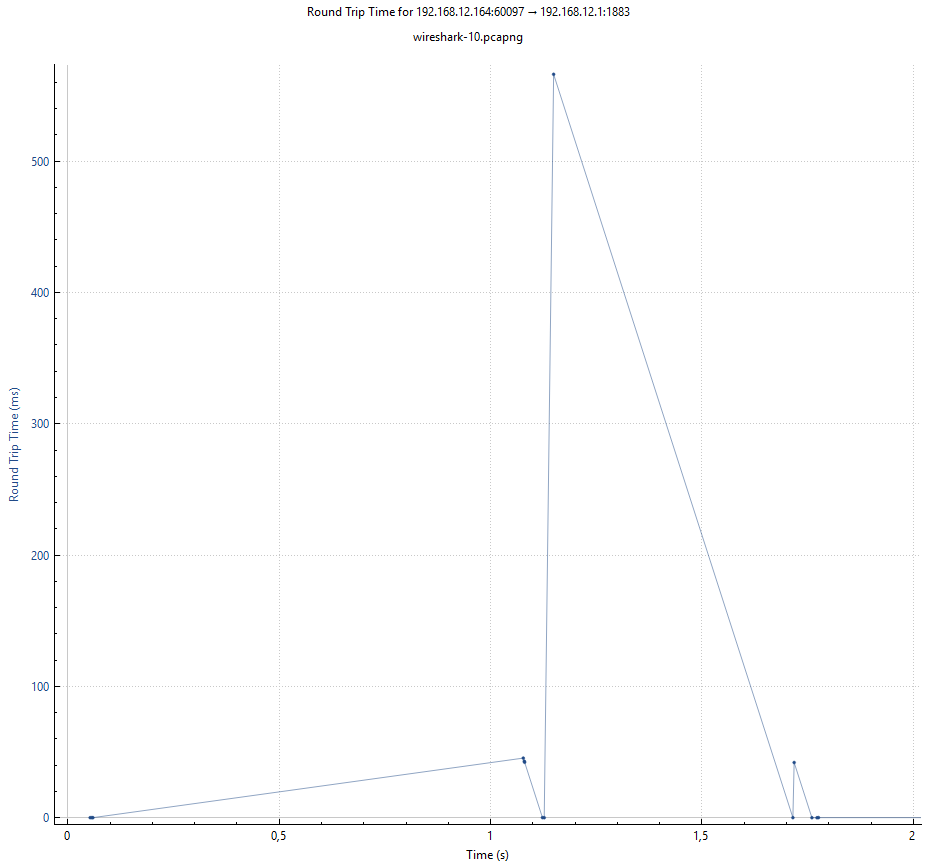
\includegraphics[width=\textwidth]{abbildungen/wireshark/10-g1.png}
    \caption{\ac{RTT} of Guardian 1 (192.168.12.164) at the start of Capture 10}
    \label{fig:rtt-g1-10}
\end{figure}
\begin{figure}[h!]
    \centering
    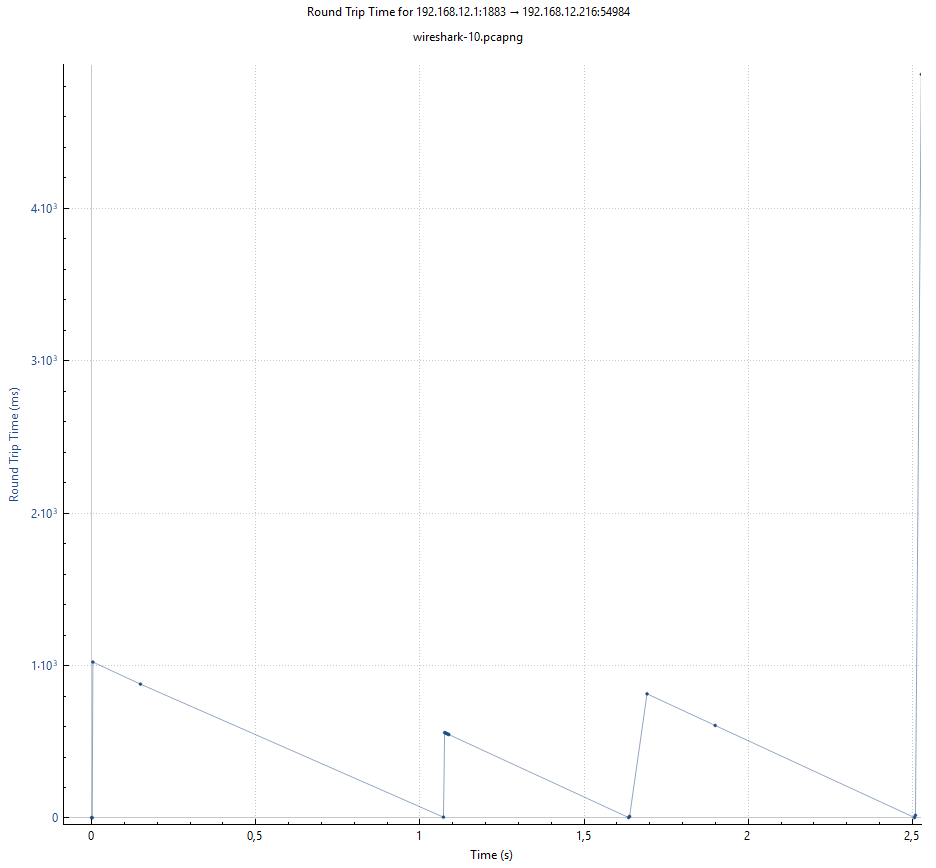
\includegraphics[width=\textwidth]{abbildungen/wireshark/10-g2.png}
    \caption{\ac{RTT} of Guardian 2 (192.168.12.164) at the start of Capture 10}
    \label{fig:rtt-g2-10}
\end{figure}
\begin{figure}[h!]
    \centering
    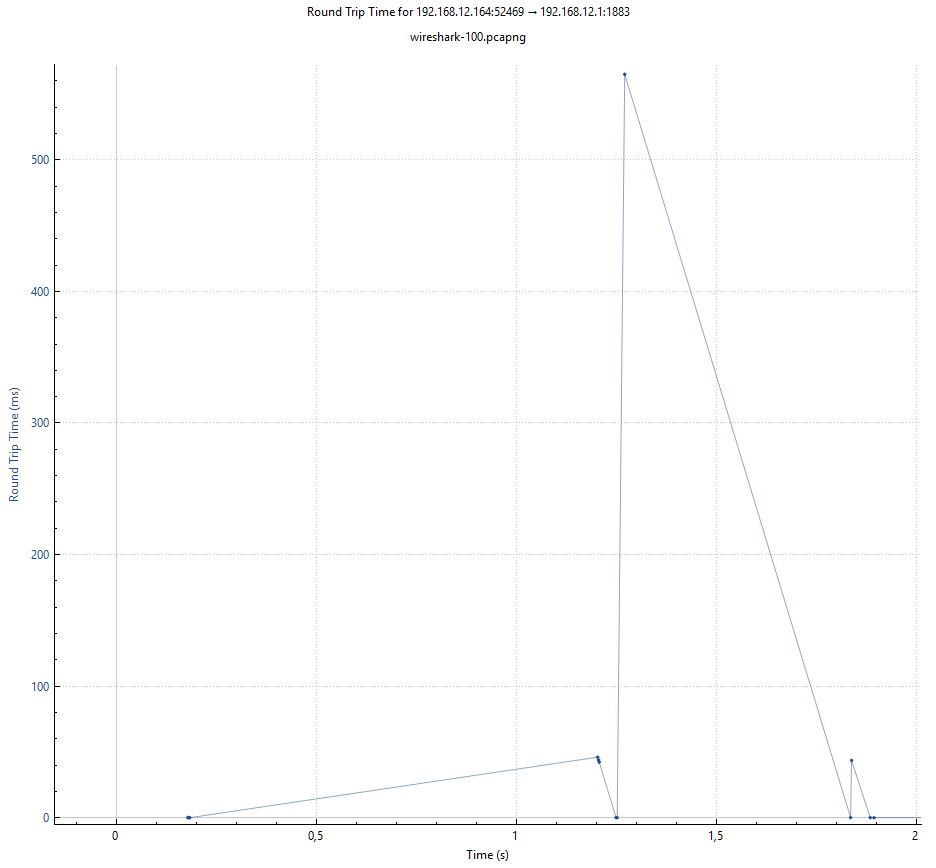
\includegraphics[width=\textwidth]{abbildungen/wireshark/100-g1.png}
    \caption{\ac{RTT} of Guardian 1 (192.168.12.164) at the start of Capture 100}
    \label{fig:rtt-g1-100}
\end{figure}
\begin{figure}[h!]
    \centering
    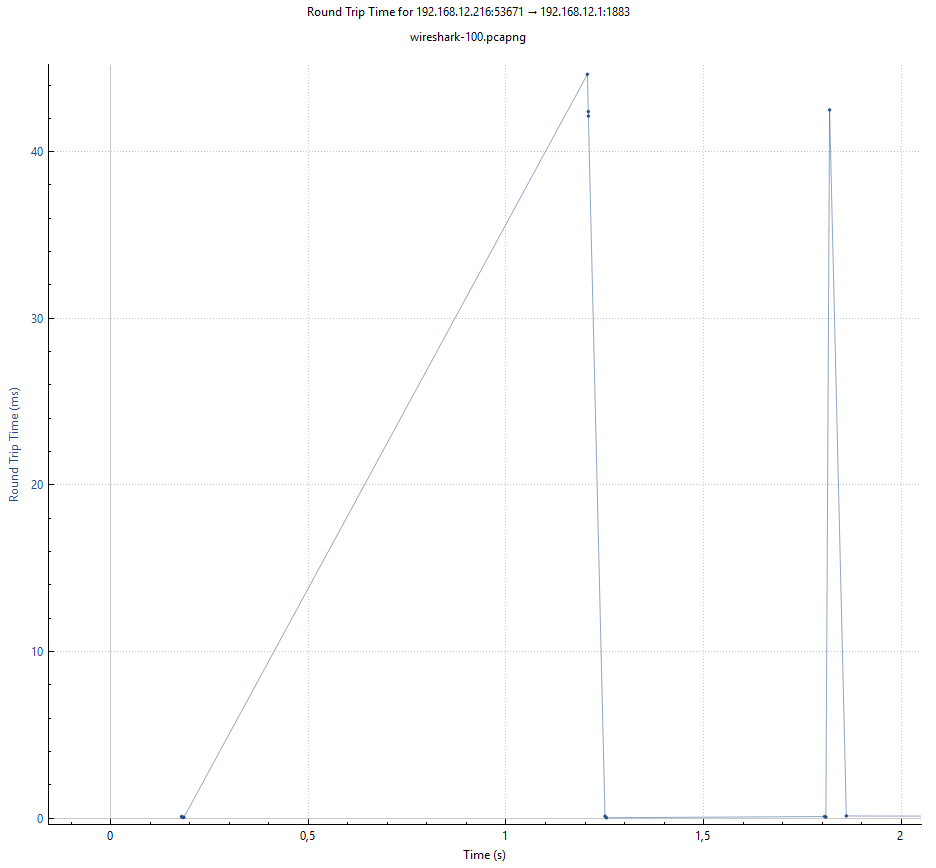
\includegraphics[width=\textwidth]{abbildungen/wireshark/100-g2.png}
    \caption{\ac{RTT} of Guardian 1 (192.168.12.164) at the start of Capture 100}
    \label{fig:rtt-g2-100}
\end{figure}
        
